\documentclass[11pt]{report}

%%  The file ``gmudissertation.sty''  is the GMU latex style file and
%%   should be placed in the same directory as your LaTeX files
\usepackage{gmudissertation}

%%
%% other packages that need to be loaded
%%
\usepackage[numbers]{natbib} % format citations
\usepackage{graphicx}                    %   for imported graphics
\usepackage{amsmath,amssymb,amsthm} %math support
\usepackage{amsfonts}                    %%  for AMS mathematics
\usepackage[normalem]{ulem}              %   a nice standard underline package
\usepackage[noadjust,verbose,sort]{cite} %   arranges reference citations neatly
\usepackage{lscape}                      % to change page orientation
\usepackage{listings}                    % to include source code
\usepackage{color}                       % for colors
\usepackage{float}              % figure placement
%% \usepackage{floatrow}

\usepackage{epstopdf} %covert .eps files to .pdf
\usepackage{curves}
\usepackage{url} %formatting for URL's
\usepackage{setspace} %change line spacing
\usepackage[mathlines]{lineno} %line numbers
\usepackage{relsize} % resize subscripts

\usepackage{tikz,pgfplots} % Creating pictures, images, cartoons, etc...
\usepackage{gnuplot-lua-tikz}
\usepackage{tikz-3dplot}
\usetikzlibrary{arrows,shapes,trees,positioning}
\usetikzlibrary{decorations.markings}
\usetikzlibrary{external} % compile figures separately
\tikzexternalize[prefix=tikz/]
\usetikzlibrary{plotmarks}

\graphicspath{{fig/}} % Location of the graphics files

\usepackage{afterpage}
\usepackage{longtable}
\usepackage[acronym]{glossaries} % create abbreviation and nomenclature lists

% decrease white space above and below caption
%% \setlength{\abovecaptionskip}{-1ex}%{-11pt}
%% \setlength{\belowcaptionskip}{-2ex}%{-8pt}


\definecolor{darkorange}{rgb}{0.9,0.3,0.0}

%%------------------------------------------------------------
%%  Abbreviations 
%%------------------------------------------------------------
%% The file ``dissertationabbrev.sty'' is an (optional) personalized file that
%% may contain any and all LaTeX command (re)definitions that will be used
%% throughout the document
\usepackage{dissertationabbrev}

%%------------------------------------------------------------
%%  Glossary
%%------------------------------------------------------------

%%------------------------------------------------------------
%%  Abbreviations
%%------------------------------------------------------------

\newacronym{aos}{AoS}{array of structures}
\newacronym{cd}{CD}{contact discontinuity}
\newacronym{clf}{CLF}{Courant-Friedrichs-Lewy}
\newacronym{ctu}{CTU}{corner transport upwind}
\newacronym{ct}{CT}{constrained transport}
\newacronym{cuda}{CUDA}{compute unified device architecture}
\newacronym{fcw}{FCW}{fast compound wave}
\newacronym{flops}{FLOPS}{floating-point operations per second}
\newacronym{fr}{FR}{fast rarefaction}
\newacronym{fs}{FS}{fast shocks}
\newacronym{fct}{FCT}{flux corrected transport}
\newacronym{fv}{FV}{finite volume}
\newacronym{gpu}{GPU}{graphics processing unit}
\newacronym{hd}{HD}{hydrodynamics}
\newacronym{hlle}{HLLE}{Harden-Lax-van Leer-Einfeldt}
\newacronym{hllc}{HLLC}{Harden-Lax-van Leer-Contact}
\newacronym{hlld}{HLLD}{Harden-Lax-van Leer-Discontinuities}
\newacronym{ivp}{IVP}{initial value problem}
\newacronym{is}{IS}{intermediate shocks}
\newacronym{mhd}{MHD}{magnetohydrodynamics}
\newacronym{ppm}{PPM}{piece-wise parabolic method}
\newacronym{omp}{OMP}{OpenMP}
\newacronym{rmse}{RMSE}{root-mean-square-error}
\newacronym{rd}{RD}{rotational discontinuity}
\newacronym{scw}{SCW}{slow compound wave}
\newacronym{soa}{SoA}{structure of arrays}
\newacronym{sr}{SR}{slow rarefaction}
\newacronym{ss}{SS}{slow shocks}
\newacronym{stl}{STL}{Standard Template Library}
\newacronym{tbb}{TBB}{thread building blocks}
\newacronym{tvd}{TVD}{total variation diminishing}
\newacronym{vl}{VL}{van Leer}

%%------------------------------------------------------------
%% Nomenclature
%%------------------------------------------------------------
\newglossaryentry{a}{
  name = $a$ ,
  description = acoustic speed of sound,
}
%% \newglossaryentry{numofangels}{
%%   name = $N$ ,
%%   description = The number of angels per needle point
%% }
%% \newglossaryentry{areaofneedle}{
%%   name = $A$ ,
%%   description = The area of the needle point
%% }

%% \makeglossaries

%% \makeglossaries % comment out to compile tikz images ///////////////////////////////////////////////
%% to update glossary: uncommented above line
%%                     compile tex document
%%                     run makeglossaries akercher_dissertation

%%------------------------------------------------------------
%%  Listing options
%%------------------------------------------------------------
\lstset{language=C++,
  basicstyle=\footnotesize\ttfamily,
  morekeywords={Point,Vector,PointArray,VectorArray},
  keywordstyle=\color{blue}\ttfamily,
  stringstyle=\color{darkred}\ttfamily,
  commentstyle=\color{darkorange}\ttfamily,
  morecomment=[l][\color{magenta}]{\#},
  breaklines=true,
  tabsize=2,
  lineskip={-1.5pt} % single line spacing
}

%**************************************************************************************************************
\begin{document}

This is a test file to preview figures.


\begin{figure}[htbp] 
\tikzsetnextfilename{coplanar_a_rsol_init_fct_1}
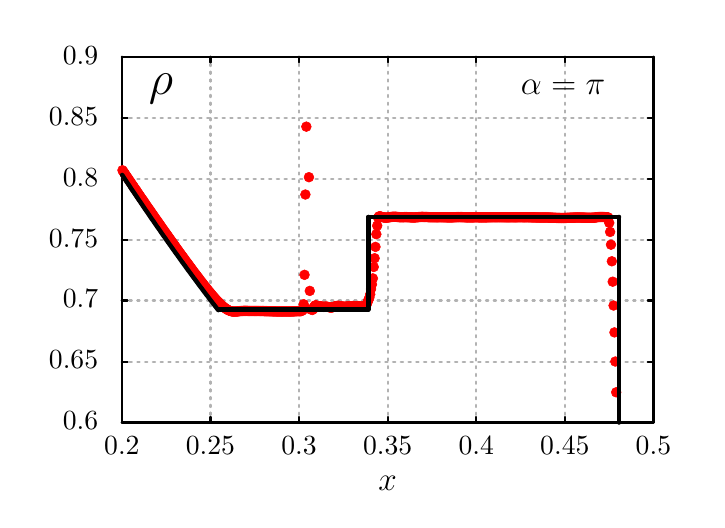
\begin{tikzpicture}[gnuplot]
%% generated with GNUPLOT 4.6p4 (Lua 5.1; terminal rev. 99, script rev. 100)
%% Sun 28 Sep 2014 07:57:49 PM EDT
\path (0.000,0.000) rectangle (8.500,6.000);
\gpfill{rgb color={1.000,1.000,1.000}} (1.196,0.985)--(7.946,0.985)--(7.946,5.630)--(1.196,5.630)--cycle;
\gpcolor{color=gp lt color border}
\gpsetlinetype{gp lt border}
\gpsetlinewidth{1.00}
\draw[gp path] (1.196,0.985)--(1.196,5.630)--(7.946,5.630)--(7.946,0.985)--cycle;
\gpcolor{color=gp lt color axes}
\gpsetlinetype{gp lt axes}
\gpsetlinewidth{2.00}
\draw[gp path] (1.196,0.985)--(7.947,0.985);
\gpcolor{color=gp lt color border}
\gpsetlinetype{gp lt border}
\draw[gp path] (1.196,0.985)--(1.268,0.985);
\draw[gp path] (7.947,0.985)--(7.875,0.985);
\gpcolor{rgb color={0.000,0.000,0.000}}
\node[gp node right,font={\fontsize{10pt}{12pt}\selectfont}] at (1.012,0.985) {0.6};
\gpcolor{color=gp lt color axes}
\gpsetlinetype{gp lt axes}
\draw[gp path] (1.196,1.759)--(7.947,1.759);
\gpcolor{color=gp lt color border}
\gpsetlinetype{gp lt border}
\draw[gp path] (1.196,1.759)--(1.268,1.759);
\draw[gp path] (7.947,1.759)--(7.875,1.759);
\gpcolor{rgb color={0.000,0.000,0.000}}
\node[gp node right,font={\fontsize{10pt}{12pt}\selectfont}] at (1.012,1.759) {0.65};
\gpcolor{color=gp lt color axes}
\gpsetlinetype{gp lt axes}
\draw[gp path] (1.196,2.534)--(7.947,2.534);
\gpcolor{color=gp lt color border}
\gpsetlinetype{gp lt border}
\draw[gp path] (1.196,2.534)--(1.268,2.534);
\draw[gp path] (7.947,2.534)--(7.875,2.534);
\gpcolor{rgb color={0.000,0.000,0.000}}
\node[gp node right,font={\fontsize{10pt}{12pt}\selectfont}] at (1.012,2.534) {0.7};
\gpcolor{color=gp lt color axes}
\gpsetlinetype{gp lt axes}
\draw[gp path] (1.196,3.308)--(7.947,3.308);
\gpcolor{color=gp lt color border}
\gpsetlinetype{gp lt border}
\draw[gp path] (1.196,3.308)--(1.268,3.308);
\draw[gp path] (7.947,3.308)--(7.875,3.308);
\gpcolor{rgb color={0.000,0.000,0.000}}
\node[gp node right,font={\fontsize{10pt}{12pt}\selectfont}] at (1.012,3.308) {0.75};
\gpcolor{color=gp lt color axes}
\gpsetlinetype{gp lt axes}
\draw[gp path] (1.196,4.082)--(7.947,4.082);
\gpcolor{color=gp lt color border}
\gpsetlinetype{gp lt border}
\draw[gp path] (1.196,4.082)--(1.268,4.082);
\draw[gp path] (7.947,4.082)--(7.875,4.082);
\gpcolor{rgb color={0.000,0.000,0.000}}
\node[gp node right,font={\fontsize{10pt}{12pt}\selectfont}] at (1.012,4.082) {0.8};
\gpcolor{color=gp lt color axes}
\gpsetlinetype{gp lt axes}
\draw[gp path] (1.196,4.857)--(7.947,4.857);
\gpcolor{color=gp lt color border}
\gpsetlinetype{gp lt border}
\draw[gp path] (1.196,4.857)--(1.268,4.857);
\draw[gp path] (7.947,4.857)--(7.875,4.857);
\gpcolor{rgb color={0.000,0.000,0.000}}
\node[gp node right,font={\fontsize{10pt}{12pt}\selectfont}] at (1.012,4.857) {0.85};
\gpcolor{color=gp lt color axes}
\gpsetlinetype{gp lt axes}
\draw[gp path] (1.196,5.631)--(7.947,5.631);
\gpcolor{color=gp lt color border}
\gpsetlinetype{gp lt border}
\draw[gp path] (1.196,5.631)--(1.268,5.631);
\draw[gp path] (7.947,5.631)--(7.875,5.631);
\gpcolor{rgb color={0.000,0.000,0.000}}
\node[gp node right,font={\fontsize{10pt}{12pt}\selectfont}] at (1.012,5.631) {0.9};
\gpcolor{color=gp lt color axes}
\gpsetlinetype{gp lt axes}
\draw[gp path] (1.196,0.985)--(1.196,5.631);
\gpcolor{color=gp lt color border}
\gpsetlinetype{gp lt border}
\draw[gp path] (1.196,0.985)--(1.196,1.057);
\draw[gp path] (1.196,5.631)--(1.196,5.559);
\gpcolor{rgb color={0.000,0.000,0.000}}
\node[gp node center,font={\fontsize{10pt}{12pt}\selectfont}] at (1.196,0.677) {0.2};
\gpcolor{color=gp lt color axes}
\gpsetlinetype{gp lt axes}
\draw[gp path] (2.321,0.985)--(2.321,5.631);
\gpcolor{color=gp lt color border}
\gpsetlinetype{gp lt border}
\draw[gp path] (2.321,0.985)--(2.321,1.057);
\draw[gp path] (2.321,5.631)--(2.321,5.559);
\gpcolor{rgb color={0.000,0.000,0.000}}
\node[gp node center,font={\fontsize{10pt}{12pt}\selectfont}] at (2.321,0.677) {0.25};
\gpcolor{color=gp lt color axes}
\gpsetlinetype{gp lt axes}
\draw[gp path] (3.446,0.985)--(3.446,5.631);
\gpcolor{color=gp lt color border}
\gpsetlinetype{gp lt border}
\draw[gp path] (3.446,0.985)--(3.446,1.057);
\draw[gp path] (3.446,5.631)--(3.446,5.559);
\gpcolor{rgb color={0.000,0.000,0.000}}
\node[gp node center,font={\fontsize{10pt}{12pt}\selectfont}] at (3.446,0.677) {0.3};
\gpcolor{color=gp lt color axes}
\gpsetlinetype{gp lt axes}
\draw[gp path] (4.572,0.985)--(4.572,5.631);
\gpcolor{color=gp lt color border}
\gpsetlinetype{gp lt border}
\draw[gp path] (4.572,0.985)--(4.572,1.057);
\draw[gp path] (4.572,5.631)--(4.572,5.559);
\gpcolor{rgb color={0.000,0.000,0.000}}
\node[gp node center,font={\fontsize{10pt}{12pt}\selectfont}] at (4.572,0.677) {0.35};
\gpcolor{color=gp lt color axes}
\gpsetlinetype{gp lt axes}
\draw[gp path] (5.697,0.985)--(5.697,5.631);
\gpcolor{color=gp lt color border}
\gpsetlinetype{gp lt border}
\draw[gp path] (5.697,0.985)--(5.697,1.057);
\draw[gp path] (5.697,5.631)--(5.697,5.559);
\gpcolor{rgb color={0.000,0.000,0.000}}
\node[gp node center,font={\fontsize{10pt}{12pt}\selectfont}] at (5.697,0.677) {0.4};
\gpcolor{color=gp lt color axes}
\gpsetlinetype{gp lt axes}
\draw[gp path] (6.822,0.985)--(6.822,5.631);
\gpcolor{color=gp lt color border}
\gpsetlinetype{gp lt border}
\draw[gp path] (6.822,0.985)--(6.822,1.057);
\draw[gp path] (6.822,5.631)--(6.822,5.559);
\gpcolor{rgb color={0.000,0.000,0.000}}
\node[gp node center,font={\fontsize{10pt}{12pt}\selectfont}] at (6.822,0.677) {0.45};
\gpcolor{color=gp lt color axes}
\gpsetlinetype{gp lt axes}
\draw[gp path] (7.947,0.985)--(7.947,5.631);
\gpcolor{color=gp lt color border}
\gpsetlinetype{gp lt border}
\draw[gp path] (7.947,0.985)--(7.947,1.057);
\draw[gp path] (7.947,5.631)--(7.947,5.559);
\gpcolor{rgb color={0.000,0.000,0.000}}
\node[gp node center,font={\fontsize{10pt}{12pt}\selectfont}] at (7.947,0.677) {0.5};
\gpcolor{color=gp lt color border}
\draw[gp path] (1.196,5.631)--(1.196,0.985)--(7.947,0.985)--(7.947,5.631)--cycle;
\gpcolor{rgb color={0.000,0.000,0.000}}
\node[gp node center,font={\fontsize{10pt}{12pt}\selectfont}] at (4.571,0.215) {\large $x$};
\gpcolor{rgb color={1.000,0.000,0.000}}
\gpsetlinewidth{0.50}
\gpsetpointsize{4.44}
\gppoint{gp mark 7}{(1.204,4.189)}
\gppoint{gp mark 7}{(1.215,4.173)}
\gppoint{gp mark 7}{(1.226,4.156)}
\gppoint{gp mark 7}{(1.237,4.140)}
\gppoint{gp mark 7}{(1.248,4.123)}
\gppoint{gp mark 7}{(1.259,4.107)}
\gppoint{gp mark 7}{(1.270,4.090)}
\gppoint{gp mark 7}{(1.282,4.074)}
\gppoint{gp mark 7}{(1.293,4.057)}
\gppoint{gp mark 7}{(1.304,4.041)}
\gppoint{gp mark 7}{(1.315,4.025)}
\gppoint{gp mark 7}{(1.326,4.008)}
\gppoint{gp mark 7}{(1.337,3.992)}
\gppoint{gp mark 7}{(1.348,3.976)}
\gppoint{gp mark 7}{(1.359,3.959)}
\gppoint{gp mark 7}{(1.371,3.943)}
\gppoint{gp mark 7}{(1.382,3.927)}
\gppoint{gp mark 7}{(1.393,3.910)}
\gppoint{gp mark 7}{(1.404,3.894)}
\gppoint{gp mark 7}{(1.415,3.878)}
\gppoint{gp mark 7}{(1.426,3.862)}
\gppoint{gp mark 7}{(1.437,3.845)}
\gppoint{gp mark 7}{(1.448,3.829)}
\gppoint{gp mark 7}{(1.460,3.813)}
\gppoint{gp mark 7}{(1.471,3.797)}
\gppoint{gp mark 7}{(1.482,3.781)}
\gppoint{gp mark 7}{(1.493,3.765)}
\gppoint{gp mark 7}{(1.504,3.748)}
\gppoint{gp mark 7}{(1.515,3.732)}
\gppoint{gp mark 7}{(1.526,3.716)}
\gppoint{gp mark 7}{(1.537,3.700)}
\gppoint{gp mark 7}{(1.548,3.684)}
\gppoint{gp mark 7}{(1.560,3.668)}
\gppoint{gp mark 7}{(1.571,3.652)}
\gppoint{gp mark 7}{(1.582,3.636)}
\gppoint{gp mark 7}{(1.593,3.620)}
\gppoint{gp mark 7}{(1.604,3.604)}
\gppoint{gp mark 7}{(1.615,3.588)}
\gppoint{gp mark 7}{(1.626,3.572)}
\gppoint{gp mark 7}{(1.637,3.556)}
\gppoint{gp mark 7}{(1.649,3.540)}
\gppoint{gp mark 7}{(1.660,3.524)}
\gppoint{gp mark 7}{(1.671,3.509)}
\gppoint{gp mark 7}{(1.682,3.493)}
\gppoint{gp mark 7}{(1.693,3.477)}
\gppoint{gp mark 7}{(1.704,3.461)}
\gppoint{gp mark 7}{(1.715,3.445)}
\gppoint{gp mark 7}{(1.726,3.429)}
\gppoint{gp mark 7}{(1.737,3.414)}
\gppoint{gp mark 7}{(1.749,3.398)}
\gppoint{gp mark 7}{(1.760,3.382)}
\gppoint{gp mark 7}{(1.771,3.367)}
\gppoint{gp mark 7}{(1.782,3.351)}
\gppoint{gp mark 7}{(1.793,3.335)}
\gppoint{gp mark 7}{(1.804,3.320)}
\gppoint{gp mark 7}{(1.815,3.304)}
\gppoint{gp mark 7}{(1.826,3.288)}
\gppoint{gp mark 7}{(1.838,3.273)}
\gppoint{gp mark 7}{(1.849,3.257)}
\gppoint{gp mark 7}{(1.860,3.242)}
\gppoint{gp mark 7}{(1.871,3.226)}
\gppoint{gp mark 7}{(1.882,3.211)}
\gppoint{gp mark 7}{(1.893,3.195)}
\gppoint{gp mark 7}{(1.904,3.180)}
\gppoint{gp mark 7}{(1.915,3.165)}
\gppoint{gp mark 7}{(1.926,3.149)}
\gppoint{gp mark 7}{(1.938,3.134)}
\gppoint{gp mark 7}{(1.949,3.118)}
\gppoint{gp mark 7}{(1.960,3.103)}
\gppoint{gp mark 7}{(1.971,3.088)}
\gppoint{gp mark 7}{(1.982,3.073)}
\gppoint{gp mark 7}{(1.993,3.057)}
\gppoint{gp mark 7}{(2.004,3.042)}
\gppoint{gp mark 7}{(2.015,3.027)}
\gppoint{gp mark 7}{(2.027,3.012)}
\gppoint{gp mark 7}{(2.038,2.997)}
\gppoint{gp mark 7}{(2.049,2.982)}
\gppoint{gp mark 7}{(2.060,2.967)}
\gppoint{gp mark 7}{(2.071,2.952)}
\gppoint{gp mark 7}{(2.082,2.937)}
\gppoint{gp mark 7}{(2.093,2.922)}
\gppoint{gp mark 7}{(2.104,2.907)}
\gppoint{gp mark 7}{(2.115,2.892)}
\gppoint{gp mark 7}{(2.127,2.877)}
\gppoint{gp mark 7}{(2.138,2.863)}
\gppoint{gp mark 7}{(2.149,2.848)}
\gppoint{gp mark 7}{(2.160,2.833)}
\gppoint{gp mark 7}{(2.171,2.819)}
\gppoint{gp mark 7}{(2.182,2.804)}
\gppoint{gp mark 7}{(2.193,2.790)}
\gppoint{gp mark 7}{(2.204,2.775)}
\gppoint{gp mark 7}{(2.216,2.761)}
\gppoint{gp mark 7}{(2.227,2.747)}
\gppoint{gp mark 7}{(2.238,2.732)}
\gppoint{gp mark 7}{(2.249,2.718)}
\gppoint{gp mark 7}{(2.260,2.704)}
\gppoint{gp mark 7}{(2.271,2.690)}
\gppoint{gp mark 7}{(2.282,2.677)}
\gppoint{gp mark 7}{(2.293,2.663)}
\gppoint{gp mark 7}{(2.304,2.649)}
\gppoint{gp mark 7}{(2.316,2.636)}
\gppoint{gp mark 7}{(2.327,2.622)}
\gppoint{gp mark 7}{(2.338,2.609)}
\gppoint{gp mark 7}{(2.349,2.596)}
\gppoint{gp mark 7}{(2.360,2.583)}
\gppoint{gp mark 7}{(2.371,2.570)}
\gppoint{gp mark 7}{(2.382,2.558)}
\gppoint{gp mark 7}{(2.393,2.545)}
\gppoint{gp mark 7}{(2.405,2.533)}
\gppoint{gp mark 7}{(2.416,2.521)}
\gppoint{gp mark 7}{(2.427,2.510)}
\gppoint{gp mark 7}{(2.438,2.498)}
\gppoint{gp mark 7}{(2.449,2.488)}
\gppoint{gp mark 7}{(2.460,2.477)}
\gppoint{gp mark 7}{(2.471,2.467)}
\gppoint{gp mark 7}{(2.482,2.457)}
\gppoint{gp mark 7}{(2.493,2.448)}
\gppoint{gp mark 7}{(2.505,2.440)}
\gppoint{gp mark 7}{(2.516,2.432)}
\gppoint{gp mark 7}{(2.527,2.425)}
\gppoint{gp mark 7}{(2.538,2.418)}
\gppoint{gp mark 7}{(2.549,2.412)}
\gppoint{gp mark 7}{(2.560,2.407)}
\gppoint{gp mark 7}{(2.571,2.403)}
\gppoint{gp mark 7}{(2.582,2.399)}
\gppoint{gp mark 7}{(2.594,2.397)}
\gppoint{gp mark 7}{(2.605,2.395)}
\gppoint{gp mark 7}{(2.616,2.395)}
\gppoint{gp mark 7}{(2.627,2.395)}
\gppoint{gp mark 7}{(2.638,2.395)}
\gppoint{gp mark 7}{(2.649,2.396)}
\gppoint{gp mark 7}{(2.660,2.396)}
\gppoint{gp mark 7}{(2.671,2.397)}
\gppoint{gp mark 7}{(2.683,2.399)}
\gppoint{gp mark 7}{(2.694,2.400)}
\gppoint{gp mark 7}{(2.705,2.401)}
\gppoint{gp mark 7}{(2.716,2.401)}
\gppoint{gp mark 7}{(2.727,2.402)}
\gppoint{gp mark 7}{(2.738,2.403)}
\gppoint{gp mark 7}{(2.749,2.403)}
\gppoint{gp mark 7}{(2.760,2.403)}
\gppoint{gp mark 7}{(2.771,2.403)}
\gppoint{gp mark 7}{(2.783,2.403)}
\gppoint{gp mark 7}{(2.794,2.403)}
\gppoint{gp mark 7}{(2.805,2.402)}
\gppoint{gp mark 7}{(2.816,2.402)}
\gppoint{gp mark 7}{(2.827,2.402)}
\gppoint{gp mark 7}{(2.838,2.402)}
\gppoint{gp mark 7}{(2.849,2.402)}
\gppoint{gp mark 7}{(2.860,2.402)}
\gppoint{gp mark 7}{(2.872,2.402)}
\gppoint{gp mark 7}{(2.883,2.402)}
\gppoint{gp mark 7}{(2.894,2.402)}
\gppoint{gp mark 7}{(2.905,2.402)}
\gppoint{gp mark 7}{(2.916,2.402)}
\gppoint{gp mark 7}{(2.927,2.402)}
\gppoint{gp mark 7}{(2.938,2.402)}
\gppoint{gp mark 7}{(2.949,2.401)}
\gppoint{gp mark 7}{(2.960,2.401)}
\gppoint{gp mark 7}{(2.972,2.401)}
\gppoint{gp mark 7}{(2.983,2.401)}
\gppoint{gp mark 7}{(2.994,2.401)}
\gppoint{gp mark 7}{(3.005,2.400)}
\gppoint{gp mark 7}{(3.016,2.400)}
\gppoint{gp mark 7}{(3.027,2.400)}
\gppoint{gp mark 7}{(3.038,2.400)}
\gppoint{gp mark 7}{(3.049,2.399)}
\gppoint{gp mark 7}{(3.061,2.399)}
\gppoint{gp mark 7}{(3.072,2.399)}
\gppoint{gp mark 7}{(3.083,2.398)}
\gppoint{gp mark 7}{(3.094,2.398)}
\gppoint{gp mark 7}{(3.105,2.398)}
\gppoint{gp mark 7}{(3.116,2.397)}
\gppoint{gp mark 7}{(3.127,2.397)}
\gppoint{gp mark 7}{(3.138,2.397)}
\gppoint{gp mark 7}{(3.149,2.397)}
\gppoint{gp mark 7}{(3.161,2.396)}
\gppoint{gp mark 7}{(3.172,2.396)}
\gppoint{gp mark 7}{(3.183,2.396)}
\gppoint{gp mark 7}{(3.194,2.396)}
\gppoint{gp mark 7}{(3.205,2.396)}
\gppoint{gp mark 7}{(3.216,2.396)}
\gppoint{gp mark 7}{(3.227,2.396)}
\gppoint{gp mark 7}{(3.238,2.396)}
\gppoint{gp mark 7}{(3.250,2.396)}
\gppoint{gp mark 7}{(3.261,2.396)}
\gppoint{gp mark 7}{(3.272,2.396)}
\gppoint{gp mark 7}{(3.283,2.396)}
\gppoint{gp mark 7}{(3.294,2.396)}
\gppoint{gp mark 7}{(3.305,2.396)}
\gppoint{gp mark 7}{(3.316,2.396)}
\gppoint{gp mark 7}{(3.327,2.396)}
\gppoint{gp mark 7}{(3.338,2.396)}
\gppoint{gp mark 7}{(3.350,2.396)}
\gppoint{gp mark 7}{(3.361,2.397)}
\gppoint{gp mark 7}{(3.372,2.397)}
\gppoint{gp mark 7}{(3.383,2.397)}
\gppoint{gp mark 7}{(3.394,2.398)}
\gppoint{gp mark 7}{(3.405,2.399)}
\gppoint{gp mark 7}{(3.416,2.399)}
\gppoint{gp mark 7}{(3.427,2.400)}
\gppoint{gp mark 7}{(3.439,2.400)}
\gppoint{gp mark 7}{(3.450,2.399)}
\gppoint{gp mark 7}{(3.461,2.400)}
\gppoint{gp mark 7}{(3.472,2.400)}
\gppoint{gp mark 7}{(3.483,2.404)}
\gppoint{gp mark 7}{(3.494,2.415)}
\gppoint{gp mark 7}{(3.505,2.488)}
\gppoint{gp mark 7}{(3.516,2.861)}
\gppoint{gp mark 7}{(3.527,3.881)}
\gppoint{gp mark 7}{(3.539,4.743)}
\gppoint{gp mark 7}{(3.572,4.101)}
\gppoint{gp mark 7}{(3.583,2.657)}
\gppoint{gp mark 7}{(3.594,2.422)}
\gppoint{gp mark 7}{(3.605,2.426)}
\gppoint{gp mark 7}{(3.616,2.415)}
\gppoint{gp mark 7}{(3.628,2.428)}
\gppoint{gp mark 7}{(3.639,2.456)}
\gppoint{gp mark 7}{(3.650,2.472)}
\gppoint{gp mark 7}{(3.661,2.474)}
\gppoint{gp mark 7}{(3.672,2.470)}
\gppoint{gp mark 7}{(3.683,2.463)}
\gppoint{gp mark 7}{(3.694,2.461)}
\gppoint{gp mark 7}{(3.705,2.461)}
\gppoint{gp mark 7}{(3.717,2.461)}
\gppoint{gp mark 7}{(3.728,2.459)}
\gppoint{gp mark 7}{(3.739,2.458)}
\gppoint{gp mark 7}{(3.750,2.456)}
\gppoint{gp mark 7}{(3.761,2.454)}
\gppoint{gp mark 7}{(3.772,2.456)}
\gppoint{gp mark 7}{(3.783,2.457)}
\gppoint{gp mark 7}{(3.794,2.457)}
\gppoint{gp mark 7}{(3.805,2.456)}
\gppoint{gp mark 7}{(3.817,2.453)}
\gppoint{gp mark 7}{(3.828,2.449)}
\gppoint{gp mark 7}{(3.839,2.447)}
\gppoint{gp mark 7}{(3.850,2.446)}
\gppoint{gp mark 7}{(3.861,2.446)}
\gppoint{gp mark 7}{(3.872,2.448)}
\gppoint{gp mark 7}{(3.883,2.453)}
\gppoint{gp mark 7}{(3.894,2.458)}
\gppoint{gp mark 7}{(3.906,2.462)}
\gppoint{gp mark 7}{(3.917,2.464)}
\gppoint{gp mark 7}{(3.928,2.466)}
\gppoint{gp mark 7}{(3.939,2.467)}
\gppoint{gp mark 7}{(3.950,2.468)}
\gppoint{gp mark 7}{(3.961,2.466)}
\gppoint{gp mark 7}{(3.972,2.463)}
\gppoint{gp mark 7}{(3.983,2.460)}
\gppoint{gp mark 7}{(3.994,2.458)}
\gppoint{gp mark 7}{(4.006,2.457)}
\gppoint{gp mark 7}{(4.017,2.457)}
\gppoint{gp mark 7}{(4.028,2.456)}
\gppoint{gp mark 7}{(4.039,2.457)}
\gppoint{gp mark 7}{(4.050,2.458)}
\gppoint{gp mark 7}{(4.061,2.459)}
\gppoint{gp mark 7}{(4.072,2.460)}
\gppoint{gp mark 7}{(4.083,2.460)}
\gppoint{gp mark 7}{(4.095,2.461)}
\gppoint{gp mark 7}{(4.106,2.462)}
\gppoint{gp mark 7}{(4.117,2.463)}
\gppoint{gp mark 7}{(4.128,2.464)}
\gppoint{gp mark 7}{(4.139,2.464)}
\gppoint{gp mark 7}{(4.150,2.464)}
\gppoint{gp mark 7}{(4.161,2.463)}
\gppoint{gp mark 7}{(4.172,2.463)}
\gppoint{gp mark 7}{(4.183,2.464)}
\gppoint{gp mark 7}{(4.195,2.464)}
\gppoint{gp mark 7}{(4.206,2.462)}
\gppoint{gp mark 7}{(4.217,2.460)}
\gppoint{gp mark 7}{(4.228,2.459)}
\gppoint{gp mark 7}{(4.239,2.458)}
\gppoint{gp mark 7}{(4.250,2.459)}
\gppoint{gp mark 7}{(4.261,2.459)}
\gppoint{gp mark 7}{(4.272,2.461)}
\gppoint{gp mark 7}{(4.284,2.465)}
\gppoint{gp mark 7}{(4.295,2.471)}
\gppoint{gp mark 7}{(4.306,2.486)}
\gppoint{gp mark 7}{(4.317,2.516)}
\gppoint{gp mark 7}{(4.328,2.542)}
\gppoint{gp mark 7}{(4.339,2.570)}
\gppoint{gp mark 7}{(4.350,2.613)}
\gppoint{gp mark 7}{(4.361,2.681)}
\gppoint{gp mark 7}{(4.372,2.740)}
\gppoint{gp mark 7}{(4.384,2.816)}
\gppoint{gp mark 7}{(4.395,2.961)}
\gppoint{gp mark 7}{(4.406,3.072)}
\gppoint{gp mark 7}{(4.417,3.216)}
\gppoint{gp mark 7}{(4.428,3.377)}
\gppoint{gp mark 7}{(4.439,3.485)}
\gppoint{gp mark 7}{(4.450,3.586)}
\gppoint{gp mark 7}{(4.461,3.603)}
\gppoint{gp mark 7}{(4.473,3.603)}
\gppoint{gp mark 7}{(4.484,3.602)}
\gppoint{gp mark 7}{(4.495,3.597)}
\gppoint{gp mark 7}{(4.506,3.594)}
\gppoint{gp mark 7}{(4.517,3.591)}
\gppoint{gp mark 7}{(4.528,3.589)}
\gppoint{gp mark 7}{(4.539,3.589)}
\gppoint{gp mark 7}{(4.550,3.588)}
\gppoint{gp mark 7}{(4.561,3.588)}
\gppoint{gp mark 7}{(4.573,3.590)}
\gppoint{gp mark 7}{(4.584,3.591)}
\gppoint{gp mark 7}{(4.595,3.593)}
\gppoint{gp mark 7}{(4.606,3.594)}
\gppoint{gp mark 7}{(4.617,3.596)}
\gppoint{gp mark 7}{(4.628,3.597)}
\gppoint{gp mark 7}{(4.639,3.598)}
\gppoint{gp mark 7}{(4.650,3.598)}
\gppoint{gp mark 7}{(4.662,3.598)}
\gppoint{gp mark 7}{(4.673,3.598)}
\gppoint{gp mark 7}{(4.684,3.597)}
\gppoint{gp mark 7}{(4.695,3.596)}
\gppoint{gp mark 7}{(4.706,3.595)}
\gppoint{gp mark 7}{(4.717,3.594)}
\gppoint{gp mark 7}{(4.728,3.593)}
\gppoint{gp mark 7}{(4.739,3.593)}
\gppoint{gp mark 7}{(4.751,3.593)}
\gppoint{gp mark 7}{(4.762,3.593)}
\gppoint{gp mark 7}{(4.773,3.593)}
\gppoint{gp mark 7}{(4.784,3.594)}
\gppoint{gp mark 7}{(4.795,3.594)}
\gppoint{gp mark 7}{(4.806,3.594)}
\gppoint{gp mark 7}{(4.817,3.594)}
\gppoint{gp mark 7}{(4.828,3.593)}
\gppoint{gp mark 7}{(4.839,3.593)}
\gppoint{gp mark 7}{(4.851,3.592)}
\gppoint{gp mark 7}{(4.862,3.591)}
\gppoint{gp mark 7}{(4.873,3.591)}
\gppoint{gp mark 7}{(4.884,3.590)}
\gppoint{gp mark 7}{(4.895,3.590)}
\gppoint{gp mark 7}{(4.906,3.590)}
\gppoint{gp mark 7}{(4.917,3.590)}
\gppoint{gp mark 7}{(4.928,3.591)}
\gppoint{gp mark 7}{(4.940,3.592)}
\gppoint{gp mark 7}{(4.951,3.593)}
\gppoint{gp mark 7}{(4.962,3.594)}
\gppoint{gp mark 7}{(4.973,3.595)}
\gppoint{gp mark 7}{(4.984,3.596)}
\gppoint{gp mark 7}{(4.995,3.596)}
\gppoint{gp mark 7}{(5.006,3.597)}
\gppoint{gp mark 7}{(5.017,3.597)}
\gppoint{gp mark 7}{(5.028,3.596)}
\gppoint{gp mark 7}{(5.040,3.596)}
\gppoint{gp mark 7}{(5.051,3.596)}
\gppoint{gp mark 7}{(5.062,3.596)}
\gppoint{gp mark 7}{(5.073,3.595)}
\gppoint{gp mark 7}{(5.084,3.594)}
\gppoint{gp mark 7}{(5.095,3.594)}
\gppoint{gp mark 7}{(5.106,3.593)}
\gppoint{gp mark 7}{(5.117,3.593)}
\gppoint{gp mark 7}{(5.129,3.593)}
\gppoint{gp mark 7}{(5.140,3.593)}
\gppoint{gp mark 7}{(5.151,3.593)}
\gppoint{gp mark 7}{(5.162,3.593)}
\gppoint{gp mark 7}{(5.173,3.593)}
\gppoint{gp mark 7}{(5.184,3.592)}
\gppoint{gp mark 7}{(5.195,3.592)}
\gppoint{gp mark 7}{(5.206,3.592)}
\gppoint{gp mark 7}{(5.217,3.593)}
\gppoint{gp mark 7}{(5.229,3.593)}
\gppoint{gp mark 7}{(5.240,3.593)}
\gppoint{gp mark 7}{(5.251,3.593)}
\gppoint{gp mark 7}{(5.262,3.593)}
\gppoint{gp mark 7}{(5.273,3.592)}
\gppoint{gp mark 7}{(5.284,3.592)}
\gppoint{gp mark 7}{(5.295,3.592)}
\gppoint{gp mark 7}{(5.306,3.592)}
\gppoint{gp mark 7}{(5.318,3.591)}
\gppoint{gp mark 7}{(5.329,3.591)}
\gppoint{gp mark 7}{(5.340,3.591)}
\gppoint{gp mark 7}{(5.351,3.591)}
\gppoint{gp mark 7}{(5.362,3.591)}
\gppoint{gp mark 7}{(5.373,3.591)}
\gppoint{gp mark 7}{(5.384,3.591)}
\gppoint{gp mark 7}{(5.395,3.591)}
\gppoint{gp mark 7}{(5.406,3.592)}
\gppoint{gp mark 7}{(5.418,3.592)}
\gppoint{gp mark 7}{(5.429,3.593)}
\gppoint{gp mark 7}{(5.440,3.593)}
\gppoint{gp mark 7}{(5.451,3.594)}
\gppoint{gp mark 7}{(5.462,3.594)}
\gppoint{gp mark 7}{(5.473,3.594)}
\gppoint{gp mark 7}{(5.484,3.594)}
\gppoint{gp mark 7}{(5.495,3.594)}
\gppoint{gp mark 7}{(5.507,3.594)}
\gppoint{gp mark 7}{(5.518,3.594)}
\gppoint{gp mark 7}{(5.529,3.593)}
\gppoint{gp mark 7}{(5.540,3.593)}
\gppoint{gp mark 7}{(5.551,3.592)}
\gppoint{gp mark 7}{(5.562,3.592)}
\gppoint{gp mark 7}{(5.573,3.591)}
\gppoint{gp mark 7}{(5.584,3.591)}
\gppoint{gp mark 7}{(5.595,3.591)}
\gppoint{gp mark 7}{(5.607,3.591)}
\gppoint{gp mark 7}{(5.618,3.591)}
\gppoint{gp mark 7}{(5.629,3.591)}
\gppoint{gp mark 7}{(5.640,3.591)}
\gppoint{gp mark 7}{(5.651,3.591)}
\gppoint{gp mark 7}{(5.662,3.591)}
\gppoint{gp mark 7}{(5.673,3.592)}
\gppoint{gp mark 7}{(5.684,3.592)}
\gppoint{gp mark 7}{(5.696,3.592)}
\gppoint{gp mark 7}{(5.707,3.592)}
\gppoint{gp mark 7}{(5.718,3.592)}
\gppoint{gp mark 7}{(5.729,3.591)}
\gppoint{gp mark 7}{(5.740,3.591)}
\gppoint{gp mark 7}{(5.751,3.591)}
\gppoint{gp mark 7}{(5.762,3.591)}
\gppoint{gp mark 7}{(5.773,3.591)}
\gppoint{gp mark 7}{(5.785,3.591)}
\gppoint{gp mark 7}{(5.796,3.591)}
\gppoint{gp mark 7}{(5.807,3.591)}
\gppoint{gp mark 7}{(5.818,3.591)}
\gppoint{gp mark 7}{(5.829,3.591)}
\gppoint{gp mark 7}{(5.840,3.592)}
\gppoint{gp mark 7}{(5.851,3.592)}
\gppoint{gp mark 7}{(5.862,3.592)}
\gppoint{gp mark 7}{(5.873,3.592)}
\gppoint{gp mark 7}{(5.885,3.592)}
\gppoint{gp mark 7}{(5.896,3.593)}
\gppoint{gp mark 7}{(5.907,3.593)}
\gppoint{gp mark 7}{(5.918,3.593)}
\gppoint{gp mark 7}{(5.929,3.593)}
\gppoint{gp mark 7}{(5.940,3.593)}
\gppoint{gp mark 7}{(5.951,3.593)}
\gppoint{gp mark 7}{(5.962,3.593)}
\gppoint{gp mark 7}{(5.974,3.593)}
\gppoint{gp mark 7}{(5.985,3.593)}
\gppoint{gp mark 7}{(5.996,3.593)}
\gppoint{gp mark 7}{(6.007,3.593)}
\gppoint{gp mark 7}{(6.018,3.593)}
\gppoint{gp mark 7}{(6.029,3.593)}
\gppoint{gp mark 7}{(6.040,3.593)}
\gppoint{gp mark 7}{(6.051,3.592)}
\gppoint{gp mark 7}{(6.062,3.592)}
\gppoint{gp mark 7}{(6.074,3.592)}
\gppoint{gp mark 7}{(6.085,3.592)}
\gppoint{gp mark 7}{(6.096,3.592)}
\gppoint{gp mark 7}{(6.107,3.592)}
\gppoint{gp mark 7}{(6.118,3.592)}
\gppoint{gp mark 7}{(6.129,3.592)}
\gppoint{gp mark 7}{(6.140,3.592)}
\gppoint{gp mark 7}{(6.151,3.592)}
\gppoint{gp mark 7}{(6.163,3.592)}
\gppoint{gp mark 7}{(6.174,3.592)}
\gppoint{gp mark 7}{(6.185,3.592)}
\gppoint{gp mark 7}{(6.196,3.592)}
\gppoint{gp mark 7}{(6.207,3.592)}
\gppoint{gp mark 7}{(6.218,3.592)}
\gppoint{gp mark 7}{(6.229,3.593)}
\gppoint{gp mark 7}{(6.240,3.593)}
\gppoint{gp mark 7}{(6.251,3.593)}
\gppoint{gp mark 7}{(6.263,3.593)}
\gppoint{gp mark 7}{(6.274,3.593)}
\gppoint{gp mark 7}{(6.285,3.593)}
\gppoint{gp mark 7}{(6.296,3.592)}
\gppoint{gp mark 7}{(6.307,3.592)}
\gppoint{gp mark 7}{(6.318,3.592)}
\gppoint{gp mark 7}{(6.329,3.592)}
\gppoint{gp mark 7}{(6.340,3.592)}
\gppoint{gp mark 7}{(6.352,3.592)}
\gppoint{gp mark 7}{(6.363,3.592)}
\gppoint{gp mark 7}{(6.374,3.592)}
\gppoint{gp mark 7}{(6.385,3.592)}
\gppoint{gp mark 7}{(6.396,3.591)}
\gppoint{gp mark 7}{(6.407,3.591)}
\gppoint{gp mark 7}{(6.418,3.591)}
\gppoint{gp mark 7}{(6.429,3.591)}
\gppoint{gp mark 7}{(6.440,3.591)}
\gppoint{gp mark 7}{(6.452,3.590)}
\gppoint{gp mark 7}{(6.463,3.590)}
\gppoint{gp mark 7}{(6.474,3.590)}
\gppoint{gp mark 7}{(6.485,3.590)}
\gppoint{gp mark 7}{(6.496,3.589)}
\gppoint{gp mark 7}{(6.507,3.589)}
\gppoint{gp mark 7}{(6.518,3.589)}
\gppoint{gp mark 7}{(6.529,3.589)}
\gppoint{gp mark 7}{(6.541,3.589)}
\gppoint{gp mark 7}{(6.552,3.589)}
\gppoint{gp mark 7}{(6.563,3.589)}
\gppoint{gp mark 7}{(6.574,3.589)}
\gppoint{gp mark 7}{(6.585,3.589)}
\gppoint{gp mark 7}{(6.596,3.589)}
\gppoint{gp mark 7}{(6.607,3.589)}
\gppoint{gp mark 7}{(6.618,3.588)}
\gppoint{gp mark 7}{(6.629,3.588)}
\gppoint{gp mark 7}{(6.641,3.588)}
\gppoint{gp mark 7}{(6.652,3.587)}
\gppoint{gp mark 7}{(6.663,3.587)}
\gppoint{gp mark 7}{(6.674,3.586)}
\gppoint{gp mark 7}{(6.685,3.586)}
\gppoint{gp mark 7}{(6.696,3.585)}
\gppoint{gp mark 7}{(6.707,3.585)}
\gppoint{gp mark 7}{(6.718,3.584)}
\gppoint{gp mark 7}{(6.730,3.584)}
\gppoint{gp mark 7}{(6.741,3.584)}
\gppoint{gp mark 7}{(6.752,3.584)}
\gppoint{gp mark 7}{(6.763,3.583)}
\gppoint{gp mark 7}{(6.774,3.583)}
\gppoint{gp mark 7}{(6.785,3.583)}
\gppoint{gp mark 7}{(6.796,3.583)}
\gppoint{gp mark 7}{(6.807,3.583)}
\gppoint{gp mark 7}{(6.818,3.584)}
\gppoint{gp mark 7}{(6.830,3.584)}
\gppoint{gp mark 7}{(6.841,3.584)}
\gppoint{gp mark 7}{(6.852,3.585)}
\gppoint{gp mark 7}{(6.863,3.585)}
\gppoint{gp mark 7}{(6.874,3.585)}
\gppoint{gp mark 7}{(6.885,3.586)}
\gppoint{gp mark 7}{(6.896,3.587)}
\gppoint{gp mark 7}{(6.907,3.587)}
\gppoint{gp mark 7}{(6.919,3.587)}
\gppoint{gp mark 7}{(6.930,3.588)}
\gppoint{gp mark 7}{(6.941,3.588)}
\gppoint{gp mark 7}{(6.952,3.588)}
\gppoint{gp mark 7}{(6.963,3.589)}
\gppoint{gp mark 7}{(6.974,3.589)}
\gppoint{gp mark 7}{(6.985,3.589)}
\gppoint{gp mark 7}{(6.996,3.589)}
\gppoint{gp mark 7}{(7.008,3.589)}
\gppoint{gp mark 7}{(7.019,3.589)}
\gppoint{gp mark 7}{(7.030,3.588)}
\gppoint{gp mark 7}{(7.041,3.588)}
\gppoint{gp mark 7}{(7.052,3.588)}
\gppoint{gp mark 7}{(7.063,3.588)}
\gppoint{gp mark 7}{(7.074,3.587)}
\gppoint{gp mark 7}{(7.085,3.587)}
\gppoint{gp mark 7}{(7.096,3.586)}
\gppoint{gp mark 7}{(7.108,3.586)}
\gppoint{gp mark 7}{(7.119,3.586)}
\gppoint{gp mark 7}{(7.130,3.586)}
\gppoint{gp mark 7}{(7.141,3.586)}
\gppoint{gp mark 7}{(7.152,3.586)}
\gppoint{gp mark 7}{(7.163,3.586)}
\gppoint{gp mark 7}{(7.174,3.587)}
\gppoint{gp mark 7}{(7.185,3.587)}
\gppoint{gp mark 7}{(7.197,3.588)}
\gppoint{gp mark 7}{(7.208,3.589)}
\gppoint{gp mark 7}{(7.219,3.591)}
\gppoint{gp mark 7}{(7.230,3.593)}
\gppoint{gp mark 7}{(7.241,3.594)}
\gppoint{gp mark 7}{(7.252,3.595)}
\gppoint{gp mark 7}{(7.263,3.595)}
\gppoint{gp mark 7}{(7.274,3.595)}
\gppoint{gp mark 7}{(7.285,3.596)}
\gppoint{gp mark 7}{(7.297,3.596)}
\gppoint{gp mark 7}{(7.308,3.595)}
\gppoint{gp mark 7}{(7.319,3.595)}
\gppoint{gp mark 7}{(7.330,3.594)}
\gppoint{gp mark 7}{(7.341,3.593)}
\gppoint{gp mark 7}{(7.352,3.593)}
\gppoint{gp mark 7}{(7.363,3.593)}
\gppoint{gp mark 7}{(7.374,3.589)}
\gppoint{gp mark 7}{(7.386,3.521)}
\gppoint{gp mark 7}{(7.397,3.406)}
\gppoint{gp mark 7}{(7.408,3.244)}
\gppoint{gp mark 7}{(7.419,3.033)}
\gppoint{gp mark 7}{(7.430,2.774)}
\gppoint{gp mark 7}{(7.441,2.471)}
\gppoint{gp mark 7}{(7.452,2.130)}
\gppoint{gp mark 7}{(7.463,1.760)}
\gppoint{gp mark 7}{(7.474,1.369)}
\gpcolor{rgb color={0.000,0.000,0.000}}
\gpsetlinetype{gp lt plot 0}
\gpsetlinewidth{4.00}
\draw[gp path] (2.427,2.420)--(3.533,2.420);
\draw[gp path] (3.533,2.420)--(4.326,2.420);
\draw[gp path] (4.326,3.596)--(7.510,3.596);
\draw[gp path] (1.200,4.130)--(1.206,4.121)--(1.212,4.112)--(1.218,4.102)--(1.224,4.093)%
  --(1.230,4.084)--(1.236,4.075)--(1.242,4.066)--(1.248,4.057)--(1.254,4.047)--(1.260,4.038)%
  --(1.267,4.029)--(1.273,4.020)--(1.279,4.011)--(1.285,4.002)--(1.291,3.993)--(1.297,3.984)%
  --(1.303,3.974)--(1.309,3.965)--(1.315,3.956)--(1.321,3.947)--(1.327,3.938)--(1.333,3.929)%
  --(1.339,3.920)--(1.346,3.911)--(1.352,3.902)--(1.358,3.893)--(1.364,3.884)--(1.370,3.875)%
  --(1.376,3.866)--(1.382,3.857)--(1.388,3.848)--(1.394,3.839)--(1.400,3.830)--(1.406,3.821)%
  --(1.412,3.812)--(1.418,3.803)--(1.425,3.794)--(1.431,3.785)--(1.437,3.776)--(1.443,3.767)%
  --(1.449,3.758)--(1.455,3.749)--(1.461,3.740)--(1.467,3.731)--(1.473,3.722)--(1.479,3.713)%
  --(1.485,3.704)--(1.491,3.695)--(1.497,3.686)--(1.504,3.677)--(1.510,3.668)--(1.516,3.660)%
  --(1.522,3.651)--(1.528,3.642)--(1.534,3.633)--(1.540,3.624)--(1.546,3.615)--(1.552,3.606)%
  --(1.558,3.597)--(1.564,3.589)--(1.570,3.580)--(1.576,3.571)--(1.583,3.562)--(1.589,3.553)%
  --(1.595,3.545)--(1.601,3.536)--(1.607,3.527)--(1.613,3.518)--(1.619,3.509)--(1.625,3.501)%
  --(1.631,3.492)--(1.637,3.483)--(1.643,3.474)--(1.649,3.465)--(1.656,3.457)--(1.662,3.448)%
  --(1.668,3.439)--(1.674,3.431)--(1.680,3.422)--(1.686,3.413)--(1.692,3.404)--(1.698,3.396)%
  --(1.704,3.387)--(1.710,3.378)--(1.716,3.370)--(1.722,3.361)--(1.728,3.352)--(1.735,3.344)%
  --(1.741,3.335)--(1.747,3.326)--(1.753,3.318)--(1.759,3.309)--(1.765,3.300)--(1.771,3.292)%
  --(1.777,3.283)--(1.783,3.274)--(1.789,3.266)--(1.795,3.257)--(1.801,3.249)--(1.807,3.240)%
  --(1.814,3.232)--(1.820,3.223)--(1.826,3.214)--(1.832,3.206)--(1.838,3.197)--(1.844,3.189)%
  --(1.850,3.180)--(1.856,3.172)--(1.862,3.163)--(1.868,3.155)--(1.874,3.146)--(1.880,3.138)%
  --(1.886,3.129)--(1.893,3.121)--(1.899,3.112)--(1.905,3.104)--(1.911,3.095)--(1.917,3.087)%
  --(1.923,3.078)--(1.929,3.070)--(1.935,3.061)--(1.941,3.053)--(1.947,3.045)--(1.953,3.036)%
  --(1.959,3.028)--(1.965,3.019)--(1.972,3.011)--(1.978,3.003)--(1.984,2.994)--(1.990,2.986)%
  --(1.996,2.978)--(2.002,2.969)--(2.008,2.961)--(2.014,2.952)--(2.020,2.944)--(2.026,2.936)%
  --(2.032,2.928)--(2.038,2.919)--(2.044,2.911)--(2.051,2.903)--(2.057,2.894)--(2.063,2.886)%
  --(2.069,2.878)--(2.075,2.869)--(2.081,2.861)--(2.087,2.853)--(2.093,2.845)--(2.099,2.837)%
  --(2.105,2.828)--(2.111,2.820)--(2.117,2.812)--(2.124,2.804)--(2.130,2.795)--(2.136,2.787)%
  --(2.142,2.779)--(2.148,2.771)--(2.154,2.763)--(2.160,2.755)--(2.166,2.746)--(2.172,2.738)%
  --(2.178,2.730)--(2.184,2.722)--(2.190,2.714)--(2.196,2.706)--(2.203,2.698)--(2.209,2.690)%
  --(2.215,2.682)--(2.221,2.673)--(2.227,2.665)--(2.233,2.657)--(2.239,2.649)--(2.245,2.641)%
  --(2.251,2.633)--(2.257,2.625)--(2.263,2.617)--(2.269,2.609)--(2.275,2.601)--(2.282,2.593)%
  --(2.288,2.585)--(2.294,2.577)--(2.300,2.569)--(2.306,2.561)--(2.312,2.553)--(2.318,2.545)%
  --(2.324,2.537)--(2.330,2.529)--(2.336,2.522)--(2.342,2.514)--(2.348,2.506)--(2.354,2.498)%
  --(2.361,2.490)--(2.367,2.482)--(2.373,2.474)--(2.379,2.466)--(2.385,2.459)--(2.391,2.451)%
  --(2.397,2.443)--(2.403,2.435)--(2.409,2.427)--(2.415,2.419)--(2.421,2.412)--(2.427,2.420);
\draw[gp path] (4.326,2.420)--(4.326,3.596);
\draw[gp path] (7.510,3.596)--(7.510,0.985);
\node[gp node left,font={\fontsize{10pt}{12pt}\selectfont}] at (1.421,5.244) {\LARGE $\rho$};
\node[gp node left,font={\fontsize{10pt}{12pt}\selectfont}] at (6.147,5.244) {\large $\alpha = \pi$};
%% coordinates of the plot area
\gpdefrectangularnode{gp plot 1}{\pgfpoint{1.196cm}{0.985cm}}{\pgfpoint{7.947cm}{5.631cm}}
\end{tikzpicture}
%% gnuplot variables

\end{figure}


\end{document}
